%-------------------------------------------------------------------------------
% seq66 sessions
%-------------------------------------------------------------------------------
%
% \file        sessions.tex
% \library     Documents
% \author      Chris Ahlstrom
% \date        2020-10-03
% \update      2023-11-24
% \version     $Revision$
% \license     $XPC_GPL_LICENSE$
%
%  Provides a discussion of how Seq66 supports session management, specifically
%  the Non Session Manager.
%
%-------------------------------------------------------------------------------

\section{Session Management}
\label{sec:sessions}

   A session is a group of applications and their configuration and
   connections.
   Session management recreate complex setups and provides some uniformity
   of application control in a session.
   The first thing to do for session management is to make sure that the
   application is capable of various levels of session management, from
   \textsl{UNIX} signals to
   a complete session manager like the \textsl{Non/New Session Manager}.
   Basic session management consist of being able to properly start the
   application and let it run properly during its life-cyle, whether it is a
   command-line application or a graphical application.
   \textsl{Seq66} supports session management in three ways:

   \begin{enumber}
      \item \textbf{Signals}.
         During a normal run, \textsl{Seq66} will respond
         to signals to save and to quit.
         The normal configuration files and command-line options will be
         used, and can be marked to be saved at exit.
         This mode is useful with \textsl{nsm-proxy}, a way to script
         applications that don't have \textsl{NSM} support.
      \item \textbf{JACK Session}
         Deprecated, but implemented nonetheless.
         Many still use it.
         This session manager allows the configuration files to be stored in
         a separate directory, for \textsl{Seq66} to be started, and files to
         be saved.  No restrictions on where the MIDI files can be stored.
      \item \textbf{Non Session Manager}
         Known as \textsl{NSM}, and in the form of a fork of that project,
         \textsl{New Session Manager},
         it provides a replacement for \textsl{JACK Session}.
         It requires all files to be
         stored in a session directory, and provides commands for saving,
         quitting, hiding/showing the user-interface, and more.
         Like \textsl{JACK Session}, it allows control over the startup of
         multiple applications, the process of saving a session, and provides a
         way to save their patching (connections) in \textsl{JACK}.
         However, it supports more functionality and has
         strict requirements the application must follow.
         Development of NSM has, for various reasons, been suspended, but
         offshoots such as \textsl{Agordejo} (\cite{agordejo})
         and \textsl{RaySession} (\cite{raysession}), which are front ends for
         the \textsl{New/Non Session Manager} (\cite{nsm}),
         continue to advance.
   \end{enumber}

   For session management, \textsl{NSM} is the way to go.
   \textsl{JACK} session management is provided for those who still use it.
   There are other session solutions, such as \textsl{aj-snapshot},
   \textsl{Claudia}, and \textsl{Chino}.
   For now, we do not discuss them.

   The desired session can be set in the \textbf{Edit / Preferences /
   Session} tab.  But note that, if started by \textsl{NSM}, \textsl{Seq66}
   will detect it and nonetheless set up for NSM usage.
   The \textsl{NSM} setting is
   useful for attaching to a pre-existing known session.
   \textsl{JACK} session management events are processed
   only if \textsl{JACK} is selected.
   \textsl{JACK} session management will still start \textsl{Seq66} in
   an existing session, if \textsl{JACK} is
   not selected.

   Also note that sometimes one will want the session manager to make the JACK
   connections.  In this case, go to
   \textbf{Edit / Preferences / JACK / Jack Auto-Connect}, uncheck that option,
   and restart \textsl{Seq66}.
   This option, \texttt{jack-auto-connect}
   can also be changed in the 'rc' file.
   The \textsl{NSM} tool called \textsl{jackpatch} can also be used to manage
   connections.

\subsection{Session Management / Signals}
\label{subsec:sessions_signals}

   \index{sessions!signals}
   By default, the basic form of session management in
   \textsl{Seq66} occurs by signals.  A
   session manager can start \textsl{Seq66}, and it can tell \textsl{Seq66} to
   save or stop.  Starting is done by a system call to spawn the application.
   The save and stop actions are supported by sending the following signals to
   the application:

   \begin{itemize}
      \item \texttt{SIGINT}.
         This signal stops \textsl{Seq66}. It corresponds
         to using \texttt{Ctrl-C} from the command-line to stop \textsl{Seq66}.
         This signal should work for both the graphical and command-line
         application.  As \textsl{Seq66} shuts down, it does its normal saving
         of the current state of the configuration.
      \item \texttt{SIGTERM}.
         This signal also stops \textsl{Seq66}.  It can
         be sent by an application to exit \textsl{Seq66}.
      \item \texttt{SIGUSR1}.
         This signal tells \textsl{Seq66} to save.  This
         action will save the current MIDI file.
   \end{itemize}

   One application that can control \textsl{Seq66} via these signals, when not
   in session mode, is \textsl{nsm-proxy}:

      \url{https://non.tuxfamily.org/wiki/nsm-proxy}

   \textsl{NSM-Proxy} is a simple \textsl{NSM} client for wrapping non-NSM
   capable programs. It enables the use of programs supporting LADISH Level 0
   and 1, and programs which accept their configuration via command-line
   arguments.  There is a command-line version and a graphical version.
   More to come on how to use \texttt{nsm-proxy}.

\subsection{Session Management / JACK Session}
\label{subsec:sessions_jack}

   Although deprecated by the \textsl{JACK} authors in favor of \textsl{NSM},
   we are implementing \textsl{JACK} session (JS) management for the benefit of
   people who either do not know of \textsl{NSM} or do not want to implement or
   use it.

   \textsl{Seq66}, as a JS-aware applications, is set up to

   \begin{enumerate}
      \item Register with a JS manager.
      \item Respond to messages from the JS manager.
      \item Be startable with session information.
   \end{enumerate}

   A response to a JS message will do one of the following:

   \begin{itemize}
      \item Save the application's state into a file, where the directory is
         supplied by the session manager.
      \item Reply to the session manager with a command-line that starts the
         application, with information to restore its state, such as
         the name of the file holding its state information.
   \end{itemize}

	JS-aware clients identify themselves to the session manager by a UUID
	(unique universal identifier). The session manager provides it to
	the client application as an integer represented as a string.
   This can be passed to the session manager when registering, but
   \textsl{Seq66} just uses the value given to it (for now).

%  but should also be passed back to the client when it is restarted
%by the session manager. This is done by a command line argument to the
%application, and the format of the command line is also up to the client.

   For this discussion, we will use the \textsl{JACK} session implementation in
   the \textsl{QjackCtl} application.
   Also, read the script stored in
   \texttt{seq66/data/linux/startqjack} to set up
   \textsl{QjackCtl} to run \textsl{JACK} and kick off
   \textsl{a2jmidid}; it should be added to the \textsl{QjackCtl}
   configuration.

   Once that setup is made (installing the script and configuring
   \texttt{qjackctl}, then start \texttt{qjackctl}.
   Verify that there are a number of system audio and MIDI playback and capture
   port, \textsl{PulseAudio JACK} sinks and sources if the system uses
   \textsl{PulseAudio}, and that there are "a2j" MIDI ports for all of your USB
   hardware devices.

   Then start \textsl{Qsynth} so it uses \textsl{jack} for MIDI and
   \textsl{jack} (or \textsl{pulseaudio}) for audio.
   Then run \textsl{Seq66} with \textsl{JACK} for slave transport and for MIDI
   (either command works the same):

   \begin{verbatim}
      $ qseq66 --jack-slave --jack-midi
      $ qseq66 --jack-slave --jack
   \end{verbatim}

   Load a file, make sure its MIDI output goes to "fluidsynth" or "qsynth", and
   plays.
   In your desired location (e.g. \texttt{~/.config/seq66/sessions},
   create a new session directory (e.g. \texttt{qtest}).

   In \textsl{qjackctl}, open the \textbf{Sessions} dialog.
   Click \textbf{Save}, and choose the directory just created.
   In the dialog should appear entries for MIDI capture and playback for
   "fluidsynth" and "seq66", all the "a2j" USB devices,
   plus an entry for \textsl{JACK} client
   \textsl{seq66master} or \textsl{seq66slave} that shows
   something like:

   \begin{verbatim}
qseq66 --jack --jack-master --jack-session-uuid 84670 --home ${SESSION_DIR}
qseq66 --jack --jack-slave --jack-session-uuid 84670 --home ${SESSION_DIR}
   \end{verbatim}

   In the \textbf{Connections} dialog of \textsl{QjackCtl}, all of these ports
   will be shown in the MIDI tab, auto-connected appropriately.
   In the sessions directory that was created, will be seen an
   empty \texttt{seq66master}
   or \texttt{seq66slave} directory, and a
   \texttt{sessions.xml} configuration file containing the information shown in
   the sessions dialog.
   Exit \textsl{Seq66}, \textsl{QSynth} and \textsl{QjackCtl}
   (in that order).

   One issue is that \textsl{QSynth}
   does not support \textsl{JACK Session}.
   Try it with \textsl{Yoshimi}, which does support it.

\subsection{Seq66 Session Management / NSM}
\label{subsec:sessions_nsm}

   \index{sessions!nsm}
   The \textsl{Non Session Manager} is an API implementation for session
   management for Linux audio/MIDI.
   \textsl{NSM} clients use a well-defined
   \index{sessions!OSC}
   \textsl{OSC} protocol (\cite{osc})
   to communicate with the session management daemon.

   Note that \textsl{Non Session Manager} is in a state of suspended
   development, and has been reimplemented as a \textsl{GitHub} project,
   the \textsl{New Session Manager}.

   The applications it manages should be installed normally (that is,
   for system-wide usage, in
   \texttt{/usr/bin/} or \texttt{/usr/local/bin}).

\subsubsection{Session Management / NSM / First Run Without NSM}
\label{subsec:sessions_nsm_first_run_without_nsm}

   This section discusses what happens when \textsl{Seq66} is installed, then
   run outside of any session from the console or an application menu.
   For a discussion where \textsl{Seq66} is run for the first time under
   \textsl{NSM},
   see \sectionref{subsec:sessions_nsm_first_run_in_nsm}.

   Generally, after installing \textsl{Seq66}, or when creating a new setup
   (such as a play-list) it is good to run it normally first, to simplify
   trouble-shooting.
   This action creates the configuration files in the default location,
   \texttt{/home/user/.config/seq66}:

\begin{verbatim}
   $ qseq66 
   No 'rc' file, will create: qseq66.rc/ctrl/midi/mutes
   No 'usr' file, will create: /home/user/.config/seq66/qseq66.usr
   File exists: /home/user/.config/seq66/qseq66.rc
   Saving initial config files to session directory!
   Writing 'rc': /home/user/.config/seq66/qseq66.rc
   Writing 'ctrl': /home/user/.config/seq66/qseq66.ctrl
   Writing 'mutes': /home/user/.config/seq66/qseq66.mutes
   Writing 'usr': /home/user/.config/seq66/qseq66.usr
   . . .
\end{verbatim}

   Then exit \textsl{Seq66} to ensure the configuration files are created.
   Optionally, in this initial setup,
   one can also create a 'playlist' file and a 'drums' file, or
   copy them from:

   \begin{verbatim}
      /usr/share/seq66-0.91/data/samples
   \end{verbatim}

   to

   \begin{verbatim}
      /home/user/.config/seq66
   \end{verbatim}

   and modify them appropriately.
   Another first-time modification to consider is setting up \textsl{Seq66} to
   use the \textsl{JACK} audio/MIDI subsystem (on \textsl{Linux}).
   In the 'rc' file, look for the following line:

   \begin{verbatim}
      [jack-transport]
      jack-midi = false
   \end{verbatim}

   And change it to:

   \begin{verbatim}
      [jack-transport]
      jack-midi = true
   \end{verbatim}

   Another first-time modification to consider is using virtual ports (option
   \texttt{--manual-ports}) versus the automatic port connections
   \textsl{Seq66} normally makes.
   This setup allows the user to manually make connections between
   \textsl{Seq66} and other MIDI applications.
   In the 'rc' file, look for the following lines:

\begin{verbatim}
   [manual-ports]
   virtual-ports = false   # 'true' = manual (virtual) ALSA or JACK ports
   output-port-count = 8   # number of manual/virtual output ports
   input-port-count = 4    # number of manual/virtual input ports
\end{verbatim}

   And change the virtual-ports line to:

\begin{verbatim}
   [manual-ports]
   virtual-ports = true    # 'true' = manual (virtual) ALSA or JACK ports
\end{verbatim}

   It is then important to start \texttt{qseq66} in the normal manner again,
   and verify that everything works as expected.

   We have added a command, \textbf{File / Import / Import Project}
   command to import the configuration files from one directory into the
   current \textsl{NSM} session configuration directory.
   This import used to be automatic, but is too surprising to an unsuspecting
   user.

\subsubsection{Seq66 Session Management / NSM / Run in NSM}
\label{subsec:sessions_nsm_first_run_in_nsm}

   Note: When \textsl{Seq66} is run in \textsl{NSM} for the first time,
   a stock default configuration is saved when
   \textsl{Seq66} exits.
   This is different from earlier behavior, where the home configuration was
   imported automatically.
   Now, the user must use the
   \textbf{File / Import / Import Project...}
   command.

   For illustration, we run \textsl{NSM} from a terminal window, which can be
   very helpful when problems occur.

\begin{verbatim}
   $ non-session-manager
   [non-session-manager] Starting daemon...
   [nsmd] Session root is: /home/user/NSM Sessions
   NSM_URL=osc.udp://mycomputer.mls:19625/
   [nsmd] Listing sessions
\end{verbatim}

   \index{sessions!non-starter}
   \index{sessions!liblo library}
   If \textsl{NSM} refuses to start, make sure that the \texttt{liblo} library
   from the OSC project is installed.
   \index{sessions!/etc/hosts}
   \index{sessions!loopback interface}
   If it is installed, then check the
   \texttt{/etc/hosts} file to make sure that a loopback interface is
   defined. In some versions of \textsl{Linux}, it isn't defined properly,
   and the \textsl{NSM} daemon (\texttt{nsmd}) will not start.
   Here is an example of the loopback installed in \textsl{Debian Sid};

\begin{verbatim}
   127.0.0.1   localhost
   127.0.1.1   mycomputer.mls mycomputer
\end{verbatim}

   The NSM user-interface (not shown here) that comes up is empty at first.
   So create a session by clicking the \textsl{NSM}
   \textsl{New} button, and entering a session name
   (here, "\textbf{Seq66}") in the
   prompt that comes up.  In the console window, a couple of 
   \texttt{/nsm/server/new} \textsl{OSC} messages
   about the creation of the session appear.

\begin{verbatim}
   [non-session-manager] Sending new for: Seq66
   [nsmd] Creating new session "Seq66"
   [non-session-manager] /nsm/server/new says Created.
   [non-session-manager] /nsm/server/new says Session created
\end{verbatim}

   Next, click the \textsl{Add Client to Session}, and, since
   \texttt{qseq66} has been installed system-wide, it is in the \texttt{PATH}
   and its executable name can be entered simply: "\texttt{qseq66}".
   A number of console messages from
   \textsl{Seq66} appear, plus some messages from \textsl{NSM}.

\begin{verbatim}
   [non-session-manager] Sending add for: qseq66
   [nsmd] Process has pid: 2797436
   [nsmd] Launching qseq66
   [nsmd] Got announce from seq66
   [nsmd] Client was expected.
   [nsmd] Process has pid: 2797436
   [nsmd] The client "seq66" at "osc.udp://127.0.0.1:13318/" informs us it's
    ready to receive commands.
\end{verbatim}

   Important: the \textsl{Seq66} user-interface will not show at first.
   It is hidden so that the screen is not inundated with the windows of all the
   applications that are (eventually) running under the session.
   This is especially annoying with tiled window managers.
   In order to see the \textsl{Seq77} user-interface, click on
   the \textbf{GUI} button in the session line shown in the \textsl{NSM} window .

   Once \textsl{Seq66} is running under \textsl{NSM},
   then click the \textbf{Save}
   button at the top of the \textsl{NSM} interface in order
   to save the session information.
   This is an \textsl{important} step.
   After \textsl{Seq66} exits,
   one can see what has been created to support the session;
   the directory that \textsl{NSM}
   creates by default is \texttt{/home/user/NSM Sessions}.
   \index{nsm!old session}

\begin{verbatim}
   $ pwd
   /home/user/NSM Sessions
   $ lstree Seq66
   Seq66/
     +-- seq66.nGJDW/
     |   +-- config/
     |   |   +-- qseq66.ctrl
     |   |   +-- qseq66.drums
     |   |   +-- qseq66.mutes
     |   |   +-- qseq66.palette
     |   |   +-- qseq66.playlist
     |   |   +-- qseq66.rc
     |   |   +-- qseq66.usr
     |   +-- midi/
     +-- session.nsm
\end{verbatim}

   \textbf{Important}: If one is running a recent "New" version of the 
   \textsl{Non Session Manager}, then the session data is not stored
   in \texttt{/home/user/NSM Sessions},
   but in
   in \texttt{/home/user/.local/share/nsm},
   Thus the above would be located differently:
   \index{nsm!new session}

\begin{verbatim}
   $ cd ~/.local/share/nsm    # the value of $XDG_DATA_HOME
   Seq66/
     +-- seq66.nGJDW/
     [ the rest is the same as above ]
\end{verbatim}

   So \textsl{NSM} has created a directory with the session name we gave it:
   \texttt{Seq66}.

   \textsl{Side note: the \texttt{nsmd} daemon creates a file named after its
   process ID in \texttt{\$XDG\_RUNTIME\_DIR/nsm/d}, e.g.
   \texttt{/run/usr/1000/nsm/d/2170}.}

   Under that directory is a file, \texttt{session.nsm}, which
   contains information like the following:

\begin{verbatim}
   seq66:qseq66:nGJDW
\end{verbatim}

   The format of this text is \texttt{appname:exename:nXYZT}, where
   \texttt{XYZT} is a 4-letter randomly-generated token
   generated by \textsl{NSM}.
   Also created is a directory, \texttt{seq66.nXYZT}, which is the root of the
   \texttt{Seq66} session.

   The rest of the directories,
   \texttt{config} and \texttt{midi},
   are generated by \textsl{Seq66}
   The \texttt{config} directory is used instead of
   \texttt{/home/user/.config/seq66}) and \texttt{midi} directory
   contains new MIDI files, imported MIDI files,
   or MIDI files from a play-list.
   The new \texttt{config} directory
   contains versions of the various configuration files that will always be
   used to start up \textsl{Seq66} during the session.
   One can also add valid play-list, palette, and drums/note-mapping files to
   that directory later.

   If before running \textsl{NSM},
   one had set up a play-list file and provided the proper "MIDI
   base directory" in the 'rc' file, then all the MIDI files are copied to
   the \textsl{NSM} session \texttt{midi} directory,
   preserving all relative directories.
   When the \textsl{Non Session Manager} is started the next time, and the
   "Seq66" session is clicked, this starts \textsl{Seq66}, and the play-list can
   be seen in the \textsl{Playlist} tab.

   Note that the \textbf{Save} button on the session's row in the
   \textsl{NSM} user-interface sends a message to \textsl{Seq66}
   to tell it to save its state.

   One last thing to note is that, when viewing the MIDI ports created by
   \textsl{Seq66}, they will be named "seq66" when not in session management,
   and "seq66.nXYZT" (for example) when under session management.  This makes
   it possible to run multiple instances of \textsl{Seq66}.

\subsubsection{Session Management / NSM / Run with Remote NSM}
\label{subsec:sessions_nsm_before_using_nsm}

   As described in the \textsl{NSM} documentation, the \texttt{nsmd} daemon can
   be run stand-alone, and can also be ran on a remote computer.
   The \texttt{qseq66.usr} file can be edited to allow \textsl{Seq66} to
   use a pre-planned \textsl{NSM} and specify the URL to connect.
   Look for the following lines in the 'usr' file:

   \begin{verbatim}
      [user-session]
      session = none
      url = ""
   \end{verbatim}

   Now assume we've run the daemon as follows:

   \begin{verbatim}
      $ nsmd --osc-port 9999
      [nsmd] Session root is: /home/user/NSM Sessions
      NSM_URL=osc.udp://mycomputer.mls:9999/
   \end{verbatim}

   Change the \texttt{session} lines to allow the usage of
   \textsl{NSM} at that URL:

\begin{verbatim}
   [user-session]
   session = nsm
   url = "osc.udp://mycomputer.mls:9999"
\end{verbatim}

   The \texttt{url} is not used if running \textsl{Seq66} from the \textsl{NSM}
   GUI... the application will get the URL from the \textsl{NSM} environment.
   Note that \texttt{qseq66} can still be run outside of a
   session manager.  It will detect the absense of the session manager and run
   normally.

\subsubsection{Session Management / Sessions Tab}
\label{subsubsec:sessions_tab}

   The \textsl{Session} tab is a mostly \textsl{read-only} tab
   provided to orient the user to the setup supported by the session.
   When not running in a session, the normal configuration directory and files
   are shown.  When running in an \textsl{NSM} section, the configuration
   information received from \textsl{NSM} is displayed.
   It is meant to display information to
   help the user understand what is happening in the run.
   Two screenshots are shown below.
%  The first shows a \textbf{Session Log} pane, but this has been removed
%  as non-functional.
   The first one is a little out-of-date;
   the second one shows access to widgets to allow
   song Text information to be stored.
   (A more flexible text facility is provided in the \textbf{Events}
   tab; see \sectionref{sec:event_editor}.)

\begin{figure}[H]
   \centering 
   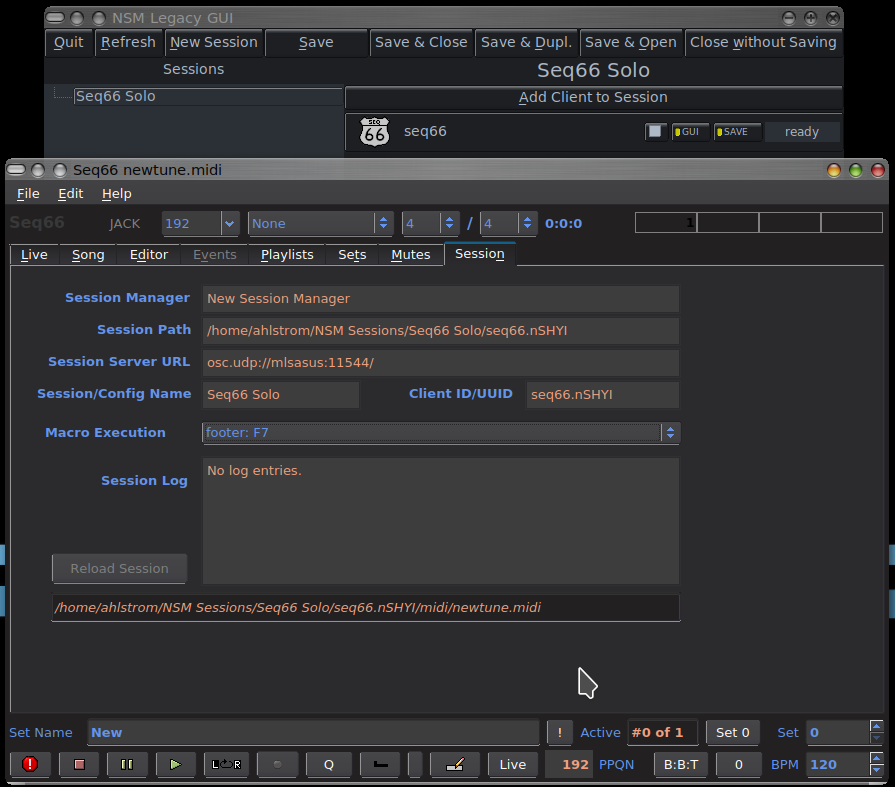
\includegraphics[scale=0.65]{tabs/session/qseq66-session-tab.png}
   \caption*{Session Tab Under NSM}
\end{figure}

   Note that the alternate coloring was set using a Qt style-sheet.
   The next diagram is more up-to-date, and shows the \textbf{Song Info}
   pane for adding a Text event to the song.

\begin{figure}[H]
   \centering 
%  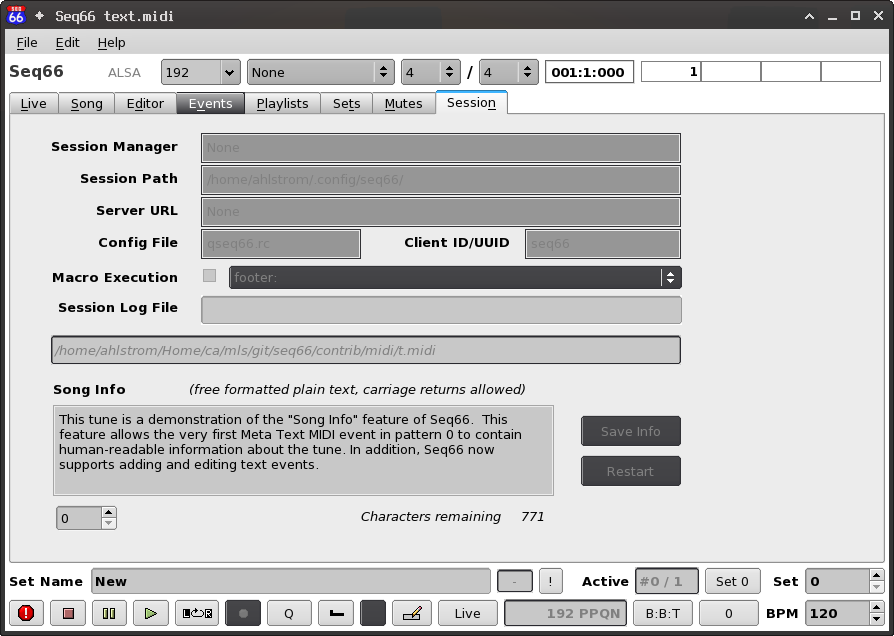
\includegraphics[scale=0.65]{tabs/session/qseq66-session-tab-song-info.png}
   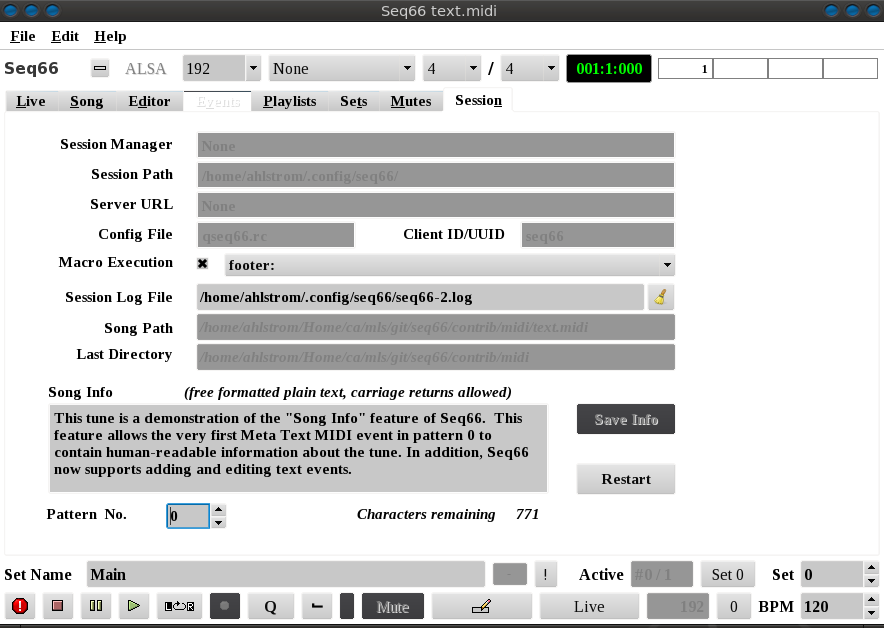
\includegraphics[scale=0.65]{tabs/session/session-song-info.png}
   \caption*{Session Tab with Song Info}
\end{figure}

   \index{sessions!ui}
   This section describes the \textsl{Session} tab in the main
   \textsl{Seq66} window.  This tab displays mostly informative and
   \textsl{read-only} information (except for the name of the log file
   and the editable song-info pane).
   It displays the following bits of information that \textsl{Seq66} has
   received from \textsl{NSM} via the \texttt{nmsd} daemon:

   \begin{itemize}
      \item \textbf{Name} of the session manager.
      \item \textbf{Session path} for the session,
         the root directory of the session.
         All data goes into this directory.
         The name of the directory is of the form
         \texttt{HOME/NSMROOT/SESSIONNAME/UNIQUEID}.
         HOME is the usual UNIX home directory for the user.
         NSMROOT depends on which version of the New/NSM session manager is
         used.
         \index{session!non}
         For the original NSM, this directory is \texttt{NSM Sessions}.
         \index{session!new}
         For the New Session Manager, this directory is
         \texttt{.local/share/nsm}.
         The session name is provided by the user when creating the
         session.
         The unique ID is generated by the NSM.
         If not running in a session,
         the active configuration directory is shown.
      \item The session's \textbf{OSC URL}, which includes the port number.
         Generally, the port number is selected at run-time, but it is also
         possible to configure \textsl{NSM} to use a specific port number.
      \item \textbf{Display name} for the session.
      \item The generated \textbf{client ID} for the session.
      \item \textbf{Macro Execution}.
         This drop-down contains all of the named MIDI macros
         defined in the 'ctrl' file's
         \texttt{[macro-control-out]} section.
         By selecting one, it is automatically sent out via the
         \texttt{[output-buss]} port defined in the 'ctrl' file.
         The "startup" and "shutdown" macros, if defined,
         are sent automatically. "Startup" is useful to put
         a MIDI controller into the proper mode for controlling and displaying
         information in \textsl{Seq66}, and "shutdown" can return the controller
         to its normal operating mode.
      \item \textbf{Session Log File}.The editable name of the log file
         to which to redirect warning
         and error messages during the of action of \textsl{qseq66}.
         Normally, the text is shown in the console window (when running in a
         console window). This name is only a base-name (e.g.
         \texttt{seq66.log}); it is always stored in HOME.
      \item \textbf{Last Directory}.
         Shows the directory from where the last MIDI file was loaded.
      \item \textbf{Restart}.
         \index{restart!manual}
         After editing some of the preferences in the \textbf{Edit / Preferences}
         dialog, one can (later)
         visit this tab and press this button to essentially
         restart \textsl{Seq66}, reloading the new configuration.
         Be careful!
      \item \textbf{Song Info} and \textbf{Pattern No.}.
         \index{song!info}
         \index{meta text}
         This item is a plaintext edit-control that allows the viewing and
         editing of "song info".
         The song info is merely the first Meta Text event, if any,
         found in pattern 0.
         The pattern number can be changed if desired, to show text in other
         patterns..
         This field can be edited with information such as date, composer,
         playback notes, etc. up to about 32000 ASCII characters.
         Extended ASCII characters are encoded as three hexadecimal
         bytes: "\\xx".
         When the \textbf{Save Info} button is clicked, the meta text
         is copied to the selected pattern, thus modifying the file, which
         can then be saved.
         For tracks (such as a karaoke lyric track) with many text events,
         they are all shown, separated by semi-colons.
         Don't try to edit such data, except in the \textsl{Event Editor}.
   \end{itemize}

   Note that there are many implementations of NSM clients:
   \textsl{Agordejo} \cite{agordejo},
   \textsl{RaySession} \cite{raysession},
   and the
   \textsl{New/Non Session Manager} \cite{nsm}
   with the JACK project's \texttt{nsm-legacy-gui}.

\subsubsection{Seq66 Session Management / NSM / File Menu}
\label{subsubsec:sessions_file_menu}

   The author of \textsl{NSM} has provided documentation for session-management
   which provides very strict instructions on how an application must behave
   under session management.  \textsl{Seq66} tries very hard to stick to these
   instructions.  One major adjustment an application must make is to adhere to
   the "File menu" guidelines.

\begin{figure}[H]
   \centering 
   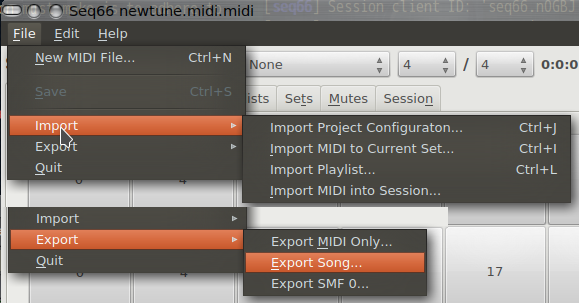
\includegraphics[scale=0.65]{tabs/session/nsm-qseq66-menus-2.png}
   \caption*{File Menu Under NSM, Composite View}
\end{figure}

   Not (yet) shown in the figure are the \textbf{Project Configuration}
   options for import and export.
   (See \sectionref{subsec:menu_file}.)

   This has been changed for 0.98.6; the \textbf{Quit} menu entry becomes
   \textbf{Hide}, as per the NSM protocol.  Also have fixed a bug that disables
   the load-most-recent option under NSM.
   We will update the figure above eventually.
   The following items describe the menu entries.

   \begin{itemize}
      \item \textbf{New MIDI File}.
         This function prompts for the name of a
         new MIDI file and clears the current MIDI file.  The file-name must not
         include a full-path to the file.  The path is hardwired by the
         session.  A relative path can be included.  This name is needed
         because there is no "Save As" option when running in an \textsl{NSM}
         session.
      \item \textbf{Import / Import Project Configuration...}
         Imports a whole project configuration into the current NSM session.
         This functionality used to be automatic (importing the "home"
         configuration), but it is better left to the user to do.
         \index{restart!automatic}
         However, the restart of \textsl{Seq66} after this operation is
         automatic.  Be careful!
      \item \textbf{Import / Import MIDI to Current Set...}
         This action works the same as in normal mode.
         This item allows the user to grab a MIDI file from anywhere and import
         it into the current set.
         The default directory that comes up in the
         prompt is the "last-used directory" from the session 'rc' file.
      \item \textbf{Import / Import Playlist...}
         This action works the same as in normal mode.
         The destination is the NSM session directory.
         \index{restart!automatic}
         Once the playlist is imported,
         \textsl{Seq66} is automatically \textsl{\textbf{restarted}}
         in order to load the playlist.
         Be careful!
      \item \textbf{Import / Import into Session...}
         Prompts the user for a MIDI file to
         be imported (copied) into the current session.  The path to the file
         is then adjusted to use the \textsl{NSM} \texttt{midi} subdirectory.
      \item \textbf{Export / Export Song...}
         Allows exporting the current song as a stock MIDI file, using the
         performance information (triggers) to write the MIDI data as it would
         be played in "song" mode.
         The default directory that comes up in the
         prompt is the "last-used directory" from the session 'rc' file.
      \item \textbf{Export / Export MIDI Only...}
         Allows exporting the current song as a stock MIDI file.
         The "proprietary" SeqSpec data is \textsl{not} written.
         The default directory that comes up in the
         prompt is the "last-used directory" from the session 'rc' file.
      \item \textbf{Export / Export SMF 0...}
         This action works the same as in normal mode.
         It converts the destination file to SMF 0 format.
      \item \textbf{Hide}.
         This menu item replaces the \textbf{Quit} item.
         It hides the main window and tells NSM about it.
   \end{itemize}

   At some point we would like to present a small tutorial showing a session
   under \textsl{JACK}.
   Also note that NSM can invoke or kill applications via
   \textsl{signals}, as explained in 
   \sectionref{subsec:sessions_signals}.

\subsubsection{Seq66 Session Management / NSM / Debugging}
\label{subsubsec:sessions_debugging}

   This section is oriented towards advanced users who found a problem running
   \textsl{Seq66} and want to track it down themselves.  The issue is that we
   need to start the application under the debugger, or start it under NSM and
   somehow attach to \textsl{Seq66} before it starts running.  Another issue is
   that we have found that, at least on the same host, an NSM session
   \textsl{must} be open before \textsl{Seq66} can attach to it, even if the
   correct \texttt{NSM\_URL} is provided.
   So we have to open a session, get the proper URL, configure it in the 'usr'
   file, and then start \textsl{Seq66} under the debugger.
   Here are the steps:

   \begin{enumerate}
      \item Start \textsl{non-session-manager} from a command-line console.
         Write down the URL that it advertises.
      \item Prepare a session for the executable as per earlier instructions.
         Once \texttt{qseq66} starts, immediately exit it, and leave the session
         open.
      \item Open the proper 'usr' file (usually \texttt{qseq66.usr}) in a 
         text editor.  Set variable "session = nsm", and set the variable "url"
         to the value that was advertised.
      \item Now start \texttt{qseq66} in a debugger.
      \item Set a breakpoint in \texttt{clinsmanager::detect\_session()}.
   \end{enumerate}
   
   Now you can step through and see where NSM and Seq66 are getting mixed up.
   Also check the session directory afterward to make the configuration
   (and any MIDI files) are in good shape.

\subsection{Seq66 Session Management / LASH}
\label{subsec:sessions_lash}

   \index{sessions!lash}
   LASH support has been removed.  Use the \textsl{NSM Session Manager} or
   the \textsl{JACK Session Manager}.

\subsection{Seq66 Session Management / sessions.rc}
\label{subsec:sessions_sessions_rc}

   \texttt{Seq66} also supports a more simplistic type of "session",
   where a whole different set of configuration files can be selected.

   One can use the \texttt{--home} and \texttt{--config} options
   to specify alternate locations and names for the configuration files.
   However, if one has a number of configurations
   (e.g. for different sets of equipment. playlists,
   style-sheets, and palettes),
   it's tedious to type these options.
   The \texttt{sessions.rc} file provides a way to set up a
   number of configurations and select one with one option.
   It is always located in the default
   "home" directory, but can refer to directories anywhere. It can also
   specify a different MIDI client-name
   (option \texttt{--client-name})
   and log-file
   (option \texttt{--option log=filename}).

   The user must manually text-edit the sessions.rc to specify tag
   sections like the following:

   \begin{verbatim}
       [test]
       home = "~/.config/seq66/test/"
       config = "test66"
       client-name = "test66"
       log = "test66.log"
   \end{verbatim}

   This section is accessed using the \texttt{-S} or
   \texttt{--session-tag} option, as shown here:

   \begin{verbatim}
       $ qseq66 --session-tag test
   \end{verbatim}

   If this is the first time this command has been run, the
   home directory is created.
   \textsl{Seq66} runs with a MIDI client-name of
   \texttt{test66}.
   The base-name of each configuration file
   is \texttt{test66} (so we have, for example, \texttt{test66.rc)}.
   The log file will be
   \texttt{~/.config/seq66/test/test66.log}.
   (If no log file is wanted, then set it to \texttt{""}.)

   At the end of the run, all of the configuration files are
   saved in 
   \texttt{~/.config/seq66/test/}.
   These can be edited to suit the "test" configuration.
   The setup can also be created via
   \textbf{File / Export / Project configure},
   and then be added to \texttt{sessions.rc}.

   The next time 
   \texttt{qseq66 --session-tag test}
   is run, the test configuration is loaded and used.

   If the specified session tag does not exist in \texttt{sessions.rc},
   then a message is shown; the user should exit \textbf{Seq66} immediately
   and fix \texttt{sessions.rc}.

   Note that the \texttt{log} option overrides the log-file setting
   present in the 'usr' file. Use \texttt{log = ""} to see console output.

%-------------------------------------------------------------------------------
% vim: ts=3 sw=3 et ft=tex
%-------------------------------------------------------------------------------
